% A schematic diagram showing the shape of the feature map as it passes through the network.

% In the encoding path, the feature map is transformed with two successive 3x3x3 convolutions and ReLU activations
% followed by a 2x2x2 max-pooling operation that reduces the spatial dimensions by half.

% In the decoding path, information from fine and coarse scales is combined through skip connections.
% The feature map is upsampled by a factor of 2 using a 3x3x3 transposed convolution.
% This is combined with the feature map from the contracting path through a skip connection,
% which is passed through an attention gate before being concatenated with the upsampled feature map.
% The feature map from deeper in the network acts as the attention gating signal.
% The upsampled feature map and attended feature map from the skip connection are concatenated and
% convolved along the channel dimension to produce the final feature map.

\documentclass{standalone}
\usepackage{tikz}
\usetikzlibrary{shapes.geometric, arrows.meta, positioning, calc}

% Styles
\tikzstyle{block} = [rectangle, draw, text centered, minimum width=2cm, minimum height=1cm, fill=white]
\tikzstyle{conv} = [thick, ->, >=stealth, black]
\tikzstyle{pool} = [thick, ->, >=stealth, blue]
\tikzstyle{up}   = [thick, ->, >=stealth, red]
\tikzstyle{skip} = [thick, dashed, ->, >=stealth, gray]
\tikzstyle{attention} = [circle, draw, text centered, minimum size=1cm, fill=orange!20]

\begin{document}
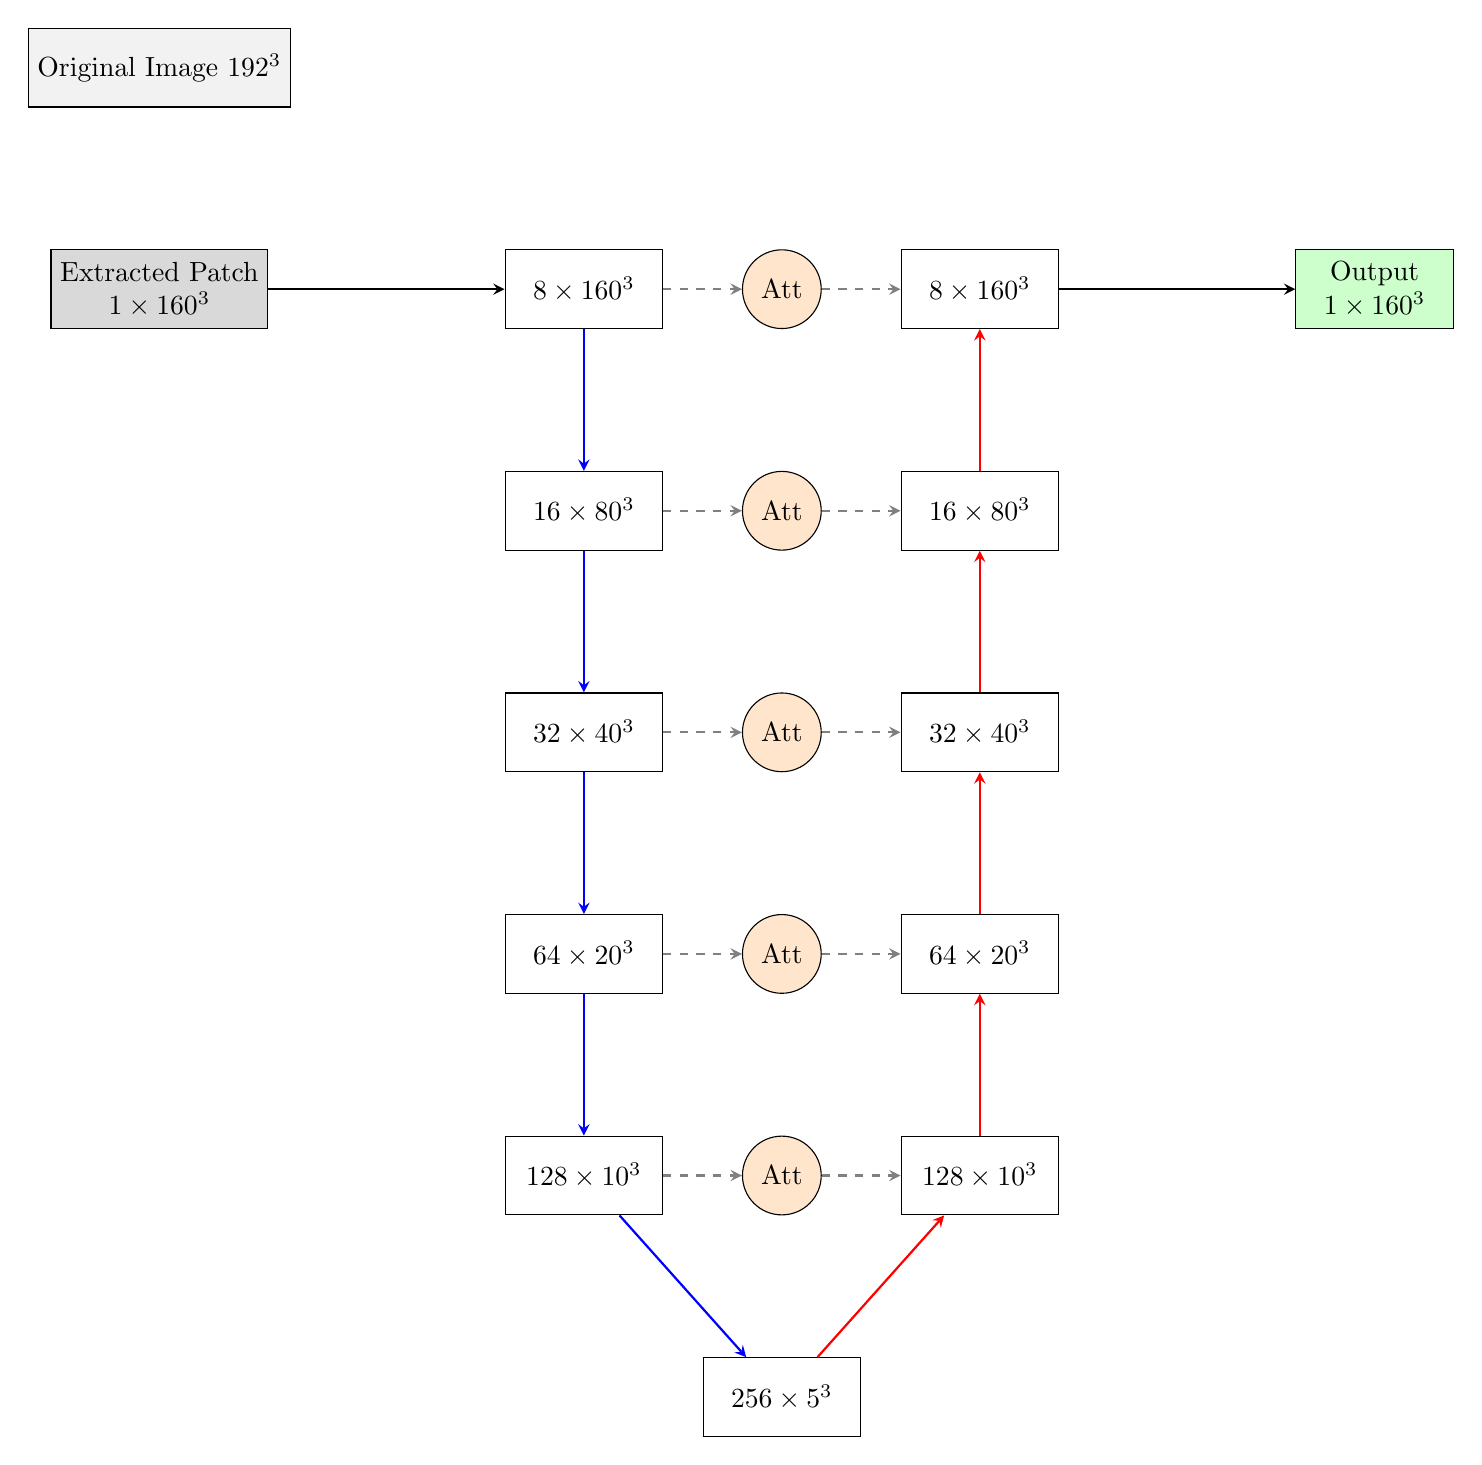
\begin{tikzpicture}[node distance=1.8cm and 0.5cm]

	% Input image and patch
	\node (input_full) [block, fill=gray!10] {Original Image $192^3$};
	\node (input_patch) [block, below=of input_full, fill=gray!30, align=center] {Extracted Patch\\$1\times160^3$};

	% Encoder
	\node (enc0) [block, right=3cm of input_patch] {$8\times160^3$};
	\node (enc1) [block, below=of enc0] {$16\times80^3$};
	\node (enc2) [block, below=of enc1] {$32\times40^3$};
	\node (enc3) [block, below=of enc2] {$64\times20^3$};
	\node (enc4) [block, below=of enc3] {$128\times10^3$};

	% Bottleneck
	\node (bottom) [block, below right=of enc4] {$256\times5^3$};

	% Decoder
	\node (dec4) [block, above right=of bottom] {$128\times10^3$};
	\node (dec3) [block, above=of dec4]   {$64\times20^3$};
	\node (dec2) [block, above=of dec3]   {$32\times40^3$};
	\node (dec1) [block, above=of dec2]   {$16\times80^3$};
	\node (dec0) [block, above=of dec1]   {$8\times160^3$};

	\node (output) [block, right=3cm of dec0, fill=green!20, align=center] {Output\\$1\times160^3$};

	% Attention Gates
	\node (att4) [attention, left=1cm of dec4] {Att};
	\node (att3) [attention, left=1cm of dec3] {Att};
	\node (att2) [attention, left=1cm of dec2] {Att};
	\node (att1) [attention, left=1cm of dec1] {Att};
	\node (att0) [attention, left=1cm of dec0] {Att};

	% Arrows - Encoder
	\draw[conv] (input_patch) -- (enc0);
	\draw[pool] (enc0) -- (enc1);
	\draw[pool] (enc1) -- (enc2);
	\draw[pool] (enc2) -- (enc3);
	\draw[pool] (enc3) -- (enc4);
	\draw[pool] (enc4) -- (bottom);

	% Arrows - Decoder
	\draw[up] (bottom) -- (dec4);
	\draw[up] (dec4) -- (dec3);
	\draw[up] (dec3) -- (dec2);
	\draw[up] (dec2) -- (dec1);
	\draw[up] (dec1) -- (dec0);
	\draw[conv] (dec0) -- (output);

	% Skip Connections with Attention
	\draw[skip] (enc4) -- (att4);
	\draw[skip] (att4) -- (dec4);
	\draw[skip] (enc3) -- (att3);
	\draw[skip] (att3) -- (dec3);
	\draw[skip] (enc2) -- (att2);
	\draw[skip] (att2) -- (dec2);
	\draw[skip] (enc1) -- (att1);
	\draw[skip] (att1) -- (dec1);
	\draw[skip] (enc0) -- (att0);
	\draw[skip] (att0) -- (dec0);

\end{tikzpicture}
\end{document}
